\documentclass{beamer}

\usepackage{geometry}
\usepackage{graphicx}
\usepackage{amsmath}

\usetheme{Boadilla}
\usepackage[utf8]{inputenc}

\useinnertheme{circles}
\newenvironment{proenv}{\only{\setbeamercolor{local structure}{fg=green}}}{}
\newenvironment{conenv}{\only{\setbeamercolor{local structure}{fg=red}}}{}

\usecolortheme{seahorse}
\setbeamertemplate{navigation symbols}{}
\title{Projet DAR : IDF Eventer}
\newcommand{\shorttitle}{M2 STL DAR}
\newcommand{\shortauthor}{16 novembre 2015}
\author{Elias Boutaleb \\ Thierry Dondon}
\date{}

\begin{document}

\usefoottemplate{\vbox{
\tinycolouredline{structure!55}%
 {\color{white}{\textbf{\shorttitle}\hfill\textbf{\shortauthor}}}%
}}

\begin{frame}
    \titlepage
\end{frame}

\begin{frame}
    \frametitle{Sommaire}
    \tableofcontents
\end{frame}

\section{Vue d'ensemble}

\begin{frame}
    \frametitle{IDF Eventer}
    \begin{center}
        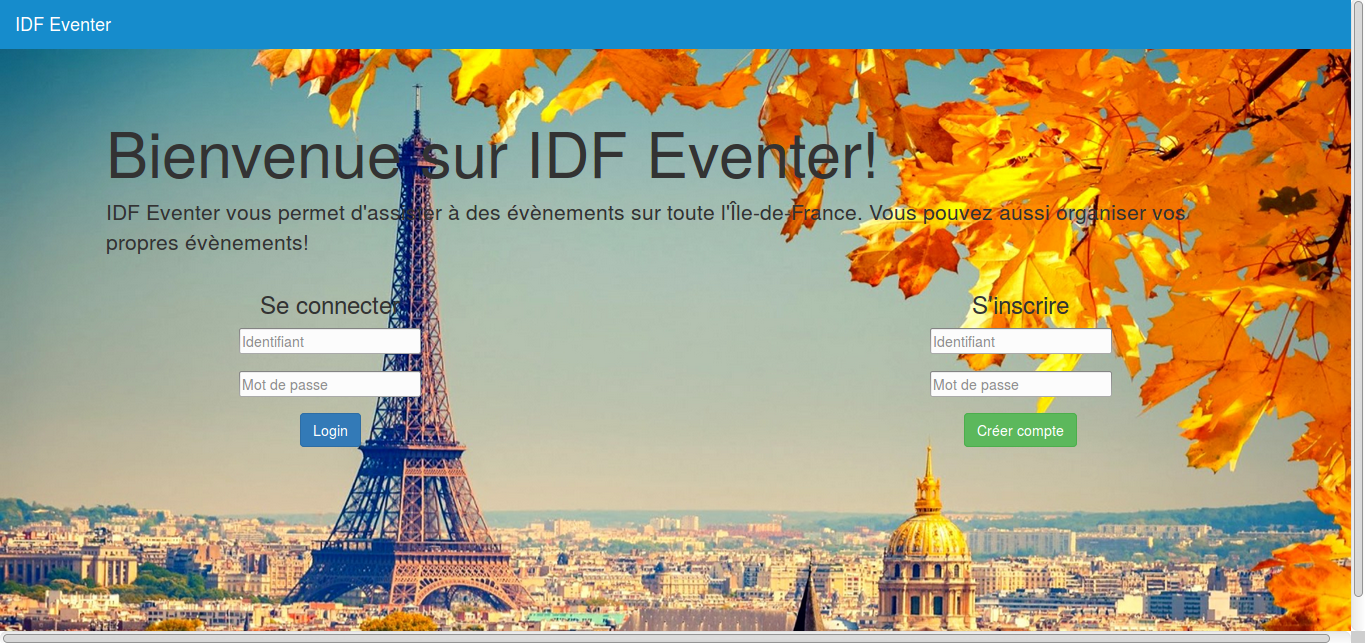
\includegraphics[scale=0.25]{../report/illus/home.png}
    \end{center}
\end{frame}

\begin{frame}
    \frametitle{Fonctionnalités}
    \begin{itemize}
        \item Voir les derniers évènements
        \item Créer son propre évènement
        \item Commenter sur un évènement
        \item S'inscrire à un évènement
        \item Voir ses inscriptions
        \item Sorties à pied/en vélo
        \begin{itemize}
            \item Tracer une route
            \item Affichage de la distance
        \end{itemize}
    \end{itemize}
\end{frame}

\section{Architecture et technologies}
\begin{frame}
    \frametitle{Schéma de l'application}
    \begin{center}
        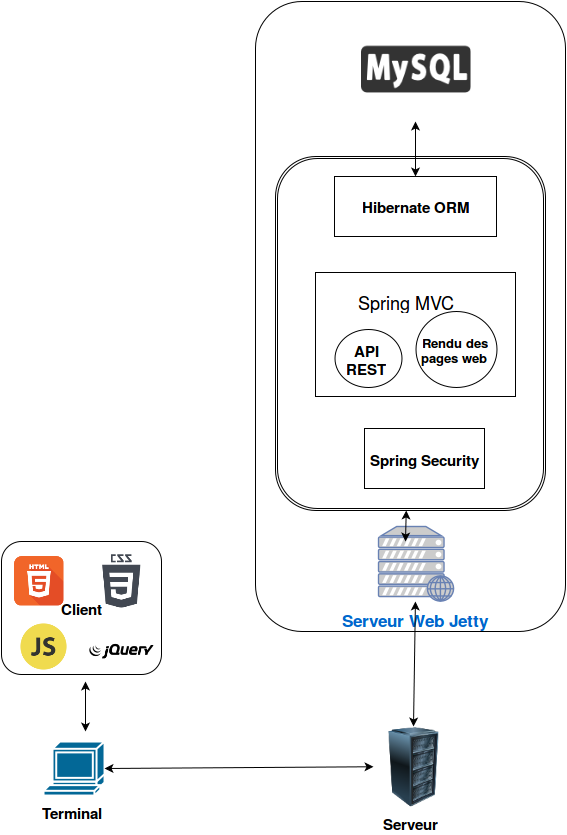
\includegraphics[scale=0.3]{../report/illus/appschema.png}
    \end{center}
\end{frame}

\begin{frame}
    \frametitle{Choix techniques}
    Côté serveur
    \begin{itemize}
        \item Serveur Web : Jetty
        \item Spring Framework (MVC + Security)
        \item Persistance des données : Hibernate + MySQL
    \end{itemize}

    Côté client
    \begin{itemize}
        \item HTML5
        \item Javascript + jQuery + jQuery UI
        \item Twitter Bootstrap
    \end{itemize}
\end{frame}


\begin{frame}
    \frametitle{Avantages et inconvénients}
    \begin{itemize}
      \item<pro@1-> Extensible \pause
      \item<pro@1-> Modulable \pause
      \item<pro@1-> Facilement déployable \pause
      \item<con@1-> Mauvais rendu sur mobile \pause
      \item<con@1-> Validation des données \pause
      \item<con@1-> Nécessité d'être inscrit et authentifié sur le site
    \end{itemize}
\end{frame}

\begin{frame}
    \frametitle{Améliorations et extensions}
    \begin{itemize}
        \item Améliorations à faire
        \begin{itemize}
            \item Rendre l’interface plus reactive
            \item Une meilleure validation des entrées (serveur et client)
        \end{itemize} \pause
        \item Extensions possibles
        \begin{itemize}
            \item Ajout d'autres types d'évènements
            \item Répertoire de lieux
            \item Système de notation des utilisateurs et évènements
            \item Recherche des évènements suivant des mots-clés
        \end{itemize}
    \end{itemize}
\end{frame}

\section{Démonstration}
\begin{frame}
    \frametitle{Démonstration}
\end{frame}

\begin{frame}
    \begin{center}
        \huge
        Merci de votre attention!\\ \pause
        \vspace{1cm}
        Des questions?
    \end{center}
\end{frame}

\end{document}
